
\documentclass[times,singlecolumn]{article}
\usepackage[margin=1in]{geometry}
\usepackage{amsmath}
\usepackage{amsfonts}
\usepackage{graphicx}
\usepackage{xcolor}
\usepackage{ulem}
\usepackage{hyperref}
% Calligraphic fonts
\newcommand{\calA}{{\cal A}}
\newcommand{\calB}{{\cal B}}
\newcommand{\calC}{{\cal C}}
\newcommand{\calD}{{\cal D}}
\newcommand{\calE}{{\cal E}}
\newcommand{\calF}{{\cal F}}
\newcommand{\calG}{{\cal G}}
\newcommand{\calH}{{\cal H}}
\newcommand{\calI}{{\cal I}}
\newcommand{\calJ}{{\cal J}}
\newcommand{\calK}{{\cal K}}
\newcommand{\calL}{{\cal L}}
\newcommand{\calM}{{\cal M}}
\newcommand{\calN}{{\cal N}}
\newcommand{\calO}{{\cal O}}
\newcommand{\calP}{{\cal P}}
\newcommand{\calQ}{{\cal Q}}
\newcommand{\calR}{{\cal R}}
\newcommand{\calS}{{\cal S}}
\newcommand{\calT}{{\cal T}}
\newcommand{\calU}{{\cal U}}
\newcommand{\calV}{{\cal V}}
\newcommand{\calW}{{\cal W}}
\newcommand{\calX}{{\cal X}}
\newcommand{\calY}{{\cal Y}}
\newcommand{\calZ}{{\cal Z}}

% Sets:
\newcommand{\setA}{\textsf{A}}
\newcommand{\setB}{\textsf{B}}
\newcommand{\setC}{\textsf{C}}
\newcommand{\setD}{\textsf{D}}
\newcommand{\setE}{\textsf{E}}
\newcommand{\setF}{\textsf{F}}
\newcommand{\setG}{\textsf{G}}
\newcommand{\setH}{\textsf{H}}
\newcommand{\setI}{\textsf{I}}
\newcommand{\setJ}{\textsf{J}}
\newcommand{\setK}{\textsf{K}}
\newcommand{\setL}{\textsf{L}}
\newcommand{\setM}{\textsf{M}}
\newcommand{\setN}{\textsf{N}}
\newcommand{\setO}{\textsf{O}}
\newcommand{\setP}{\textsf{P}}
\newcommand{\setQ}{\textsf{Q}}
\newcommand{\setR}{\textsf{R}}
\newcommand{\setS}{\textsf{S}}
\newcommand{\setT}{\textsf{T}}
\newcommand{\setU}{\textsf{U}}
\newcommand{\setV}{\textsf{V}}
\newcommand{\setW}{\textsf{W}}
\newcommand{\setX}{\textsf{X}}
\newcommand{\setY}{\textsf{Y}}
\newcommand{\setZ}{\textsf{Z}}

% Vectors
\newcommand{\bfa}{\mathbf{a}}
\newcommand{\bfb}{\mathbf{b}}
\newcommand{\bfc}{\mathbf{c}}
\newcommand{\bfd}{\mathbf{d}}
\newcommand{\bfe}{\mathbf{e}}
\newcommand{\bff}{\mathbf{f}}
\newcommand{\bfg}{\mathbf{g}}
\newcommand{\bfh}{\mathbf{h}}
\newcommand{\bfi}{\mathbf{i}}
\newcommand{\bfj}{\mathbf{j}}
\newcommand{\bfk}{\mathbf{k}}
\newcommand{\bfl}{\mathbf{l}}
\newcommand{\bfm}{\mathbf{m}}
\newcommand{\bfn}{\mathbf{n}}
\newcommand{\bfo}{\mathbf{o}}
\newcommand{\bfp}{\mathbf{p}}
\newcommand{\bfq}{\mathbf{q}}
\newcommand{\bfr}{\mathbf{r}}
\newcommand{\bfs}{\mathbf{s}}
\newcommand{\bft}{\mathbf{t}}
\newcommand{\bfu}{\mathbf{u}}
\newcommand{\bfv}{\mathbf{v}}
\newcommand{\bfw}{\mathbf{w}}
\newcommand{\bfx}{\mathbf{x}}
\newcommand{\bfy}{\mathbf{y}}
\newcommand{\bfz}{\mathbf{z}}


\newcommand{\bfalpha}{\boldsymbol{\alpha}}
\newcommand{\bfbeta}{\boldsymbol{\beta}}
\newcommand{\bfgamma}{\boldsymbol{\gamma}}
\newcommand{\bfdelta}{\boldsymbol{\delta}}
\newcommand{\bfepsilon}{\boldsymbol{\epsilon}}
\newcommand{\bfzeta}{\boldsymbol{\zeta}}
\newcommand{\bfeta}{\boldsymbol{\eta}}
\newcommand{\bftheta}{\boldsymbol{\theta}}
\newcommand{\bfiota}{\boldsymbol{\iota}}
\newcommand{\bfkappa}{\boldsymbol{\kappa}}
\newcommand{\bflambda}{\boldsymbol{\lambda}}
\newcommand{\bfmu}{\boldsymbol{\mu}}
\newcommand{\bfnu}{\boldsymbol{\nu}}
\newcommand{\bfomicron}{\boldsymbol{\omicron}}
\newcommand{\bfpi}{\boldsymbol{\pi}}
\newcommand{\bfrho}{\boldsymbol{\rho}}
\newcommand{\bfsigma}{\boldsymbol{\sigma}}
\newcommand{\bftau}{\boldsymbol{\tau}}
\newcommand{\bfupsilon}{\boldsymbol{\upsilon}}
\newcommand{\bfphi}{\boldsymbol{\phi}}
\newcommand{\bfchi}{\boldsymbol{\chi}}
\newcommand{\bfpsi}{\boldsymbol{\psi}}
\newcommand{\bfomega}{\boldsymbol{\omega}}
\newcommand{\bfxi}{\boldsymbol{\xi}}
\newcommand{\bfell}{\boldsymbol{\ell}}

% Matrices
\newcommand{\bfA}{\mathbf{A}}
\newcommand{\bfB}{\mathbf{B}}
\newcommand{\bfC}{\mathbf{C}}
\newcommand{\bfD}{\mathbf{D}}
\newcommand{\bfE}{\mathbf{E}}
\newcommand{\bfF}{\mathbf{F}}
\newcommand{\bfG}{\mathbf{G}}
\newcommand{\bfH}{\mathbf{H}}
\newcommand{\bfI}{\mathbf{I}}
\newcommand{\bfJ}{\mathbf{J}}
\newcommand{\bfK}{\mathbf{K}}
\newcommand{\bfL}{\mathbf{L}}
\newcommand{\bfM}{\mathbf{M}}
\newcommand{\bfN}{\mathbf{N}}
\newcommand{\bfO}{\mathbf{O}}
\newcommand{\bfP}{\mathbf{P}}
\newcommand{\bfQ}{\mathbf{Q}}
\newcommand{\bfR}{\mathbf{R}}
\newcommand{\bfS}{\mathbf{S}}
\newcommand{\bfT}{\mathbf{T}}
\newcommand{\bfU}{\mathbf{U}}
\newcommand{\bfV}{\mathbf{V}}
\newcommand{\bfW}{\mathbf{W}}
\newcommand{\bfX}{\mathbf{X}}
\newcommand{\bfY}{\mathbf{Y}}
\newcommand{\bfZ}{\mathbf{Z}}


\newcommand{\bfGamma}{\boldsymbol{\Gamma}}
\newcommand{\bfDelta}{\boldsymbol{\Delta}}
\newcommand{\bfTheta}{\boldsymbol{\Theta}}
\newcommand{\bfLambda}{\boldsymbol{\Lambda}}
\newcommand{\bfPi}{\boldsymbol{\Pi}}
\newcommand{\bfSigma}{\boldsymbol{\Sigma}}
\newcommand{\bfUpsilon}{\boldsymbol{\Upsilon}}
\newcommand{\bfPhi}{\boldsymbol{\Phi}}
\newcommand{\bfPsi}{\boldsymbol{\Psi}}
\newcommand{\bfOmega}{\boldsymbol{\Omega}}


% Blackboard Bold:
\newcommand{\bbA}{\mathbb{A}}
\newcommand{\bbB}{\mathbb{B}}
\newcommand{\bbC}{\mathbb{C}}
\newcommand{\bbD}{\mathbb{D}}
\newcommand{\bbE}{\mathbb{E}}
\newcommand{\bbF}{\mathbb{F}}
\newcommand{\bbG}{\mathbb{G}}
\newcommand{\bbH}{\mathbb{H}}
\newcommand{\bbI}{\mathbb{I}}
\newcommand{\bbJ}{\mathbb{J}}
\newcommand{\bbK}{\mathbb{K}}
\newcommand{\bbL}{\mathbb{L}}
\newcommand{\bbM}{\mathbb{M}}
\newcommand{\bbN}{\mathbb{N}}
\newcommand{\bbO}{\mathbb{O}}
\newcommand{\bbP}{\mathbb{P}}
\newcommand{\bbQ}{\mathbb{Q}}
\newcommand{\bbR}{\mathbb{R}}
\newcommand{\bbS}{\mathbb{S}}
\newcommand{\bbT}{\mathbb{T}}
\newcommand{\bbU}{\mathbb{U}}
\newcommand{\bbV}{\mathbb{V}}
\newcommand{\bbW}{\mathbb{W}}
\newcommand{\bbX}{\mathbb{X}}
\newcommand{\bbY}{\mathbb{Y}}
\newcommand{\bbZ}{\mathbb{Z}}





\newcommand{\ubfu}{\underline{\bfu}}
\newcommand{\ubfx}{\underline{\bfx}}

\newtheorem{prob}{Problem}


\title{ECE 417/598: K,R,t from P matrix}
\author{Instructor: Vikas Dhiman}
\DeclareMathOperator{\diag}{diag}
\begin{document}
\maketitle
\begin{tabular}{p{0.5\linewidth}p{0.5\linewidth}}
  (1) Student name:& Student email: \\
\end{tabular}

\paragraph{Rules}
\begin{enumerate}
\item Let unit vectors of $\bfa$ be denoted by $\hat{\bfa} = \frac{\bfa}{\|\bfa\|}$.
\item The projection of $\bfb$ on $\bfa$ is $\overrightarrow{PQ}$. The
  magnitude of the projection is given by dot product,
  \[ |\overrightarrow{PQ}| = \bfb^\top \hat{\bfa} = \hat{\bfa}^\top \bfb =
    \|\hat{\bfa}\|\|\bfb\|\cos(\theta) =  \|\bfb\|\cos(\theta)\]
  \item Since $\overrightarrow{PQ}$ is in the direction of $\hat{\bfa}$, the
    vector $\overrightarrow{PQ}$ is given by,
    \[
      \overrightarrow{PQ} = |\overrightarrow{PQ}| \hat{\bfa}
      = ( \bfb^\top \hat{\bfa}) \hat{\bfa}
    \]
\item Similarly the projection of $\bfb$ on $\hat{\bfc}$  is $\overrightarrow{QR}$
  \[ |\overrightarrow{QR}| = \bfb^\top \hat{\bfc} = \hat{\bfc}^\top \bfb =
    \|\hat{\bfa}\|\|\bfb\|\cos(\frac{\pi}{2} - \theta) =  \|\bfb\|\cos(\frac{\pi}{2} - \theta)\]
  \[ \overrightarrow{QR} = (\bfb^\top \hat{\bfc})  \hat{\bfc} \]
\item By triangle law $\bfb = \overrightarrow{PQ} + \overrightarrow{QR}$,
  or
  \[
    \bfb = (\bfb^\top \hat{\bfa}) \hat{\bfa} + (\bfb^\top \hat{\bfc})\hat{\bfc}
  \]

\end{enumerate}

\hfill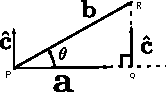
\includegraphics[width=0.25\linewidth]{media/triangle-law-projection.pdf}

\begin{prob}
\item We want to find a pair of orthonormal vectors in the same plane as $\bfa$ and $\bfb$.
  First vector is $\hat{\bfa}$. What is the second vector? (Call it $\hat{\bfc}$
  and find it in terms of $\bfa$ and $\bfb$.)
    
\end{prob}
%\hfill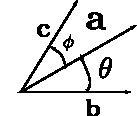
\includegraphics[width=0.25\linewidth]{media/triangle-law-2.pdf}

\newpage
\vspace{10em}
\begin{prob}
  Express the above relationship in terms of matrix vector multiplication so
  that the matrix $M = \begin{bmatrix}
    \bfb^\top \\ \bfa^\top\end{bmatrix}$ can be written in terms of an upper
  triangular matrix and an orthonormal matrix.
\end{prob}

\vspace{10em}

\newpage
\begin{prob}
  Repeat the process for 3 vectors, $\bfa$, $\bfb$ and $\bfc$, and then matrix
  $M = \begin{bmatrix} \bfc^\top \\ \bfb^\top \\ \bfa^\top\end{bmatrix}$. In
  other words, find $\hat{\bfr}_1$, $\hat{\bfr}_2$, $\hat{\bfr}_3$ and write
  them in (upper triangular matrix) (orthonormal matrix) factorization form,
  also known as QR factorization.
\end{prob}
\hfill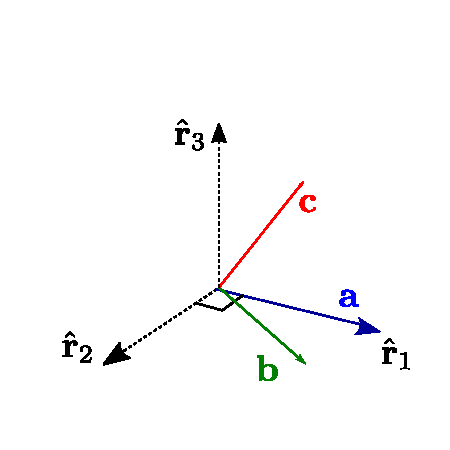
\includegraphics[width=0.5\linewidth]{media/gram-schmidt-3D.pdf}

\begin{enumerate}
  \item Write $\hat{\bfr}_1$ in terms of $\bfa$.
    \vspace{10em}
  \item Write $\hat{\bfr}_2$ in terms of $\bfa$, $\bfb$ and $\hat{\bfr}_1$.
    \vspace{10em}
  \item Write $\hat{\bfr}_3$ in terms of $\bfa$, $\bfb$, $\bfc$, $\hat{\bfr}_1$
    and $\hat{\bfr}_2$.
    \vspace{10em}

\newpage

\item Write the above equations in matrix multiplication form.
  \vspace{10em}
\end{enumerate}

\begin{prob}
  Assuming a QR factorization algorithm is given, find $K, R, \bft$ from $P \in \bbR^{3
    \times 4}$ matrix such that
  \[
  P = \begin{bmatrix}
    KR & K\bft
    \end{bmatrix}
      \]
      and $K \in \bbR^{3 \times 3}$ is an upper triangular matrix, and $R \in
      \bbR^{3 \times 3}$  is a rotation matrix (thus orthonormal) and $\bft \in
      \bbR^{3 \times 1}$ is a translation vector.
  

\end{document}